
\documentclass{article} % For LaTeX2e
\usepackage{iclr2027_conference,times}

% Optional math commands from https://github.com/goodfeli/dlbook_notation.
\input{math_commands.tex}
\newtheorem{theorem}{Theorem}
\newtheorem{corollary}{Corollary}
\newtheorem{remark}{Remark}
\newtheorem{lemma}{Lemma}
\newtheorem{proposition}{Proposition}
\usepackage{hyperref}
\usepackage{url}
\usepackage{booktabs}
\usepackage{graphicx}
\usepackage{wrapfig}
\usepackage{multirow}


\title{TH-JEPA: Temporal Hypergraph Joint-Embedding Predictive Architecture for Multi-Agent Path Finding}

% Authors must not appear in the submitted version. They should be hidden
% as long as the \iclrfinalcopy macro remains commented out below.
% Non-anonymous submissions will be rejected without review.

\author{Antiquus S.~Hippocampus, Natalia Cerebro \& Amelie P. Amygdale \thanks{ Use footnote for providing further information
about author (webpage, alternative address)---\emph{not} for acknowledging
funding agencies.  Funding acknowledgements go at the end of the paper.} \\
Department of Computer Science\\
Cranberry-Lemon University\\
Pittsburgh, PA 15213, USA \\
\texttt{\{hippo,brain,jen\}@cs.cranberry-lemon.edu} \\
\And
Ji Q. Ren \& Yevgeny LeNet \\
Department of Computational Neuroscience \\
University of the Witwatersrand \\
Joburg, South Africa \\
\texttt{\{robot,net\}@wits.ac.za} \\
\AND
Coauthor \\
Affiliation \\
Address \\
\texttt{email}
}

% The \author macro works with any number of authors. There are two commands
% used to separate the names and addresses of multiple authors: \And and \AND.
%
% Using \And between authors leaves it to \LaTeX{} to determine where to break
% the lines. Using \AND forces a linebreak at that point. So, if \LaTeX{}
% puts 3 of 4 authors names on the first line, and the last on the second
% line, try using \AND instead of \And before the third author name.

\newcommand{\fix}{\marginpar{FIX}}
\newcommand{\new}{\marginpar{NEW}}

%\iclrfinalcopy % Uncomment for camera-ready version, but NOT for submission.
\begin{document}


\maketitle

\begin{abstract}
Graphs can exhibit distinct local signal regimes, ranging from smooth
homophilous regions to sharp heterophilous boundaries. However, many GNNs rely on graph-wide propagation operators that mix these signals through a shared geometry; repeated propagation and degree imbalance can further amplify hub influence, suppress discriminative variation, and aggravate oversmoothing and long-range information bottlenecks. We propose \textbf{Hierarchical Spectral Learning (HSL)}, which combines multi-view graph geometry, diffusion-coherent hierarchical coarsening, and a degree-aware Haar decomposition to construct orthogonal, spatially localized multiresolution components with adaptive spectral filtering. Diffusion refinement improves local separation, while the hierarchy preserves fine-scale contrasts and introduces broader interactions only at progressively coarser resolutions. Theoretically, we establish depth-independent preservation of hierarchy contrast energy and explicit hierarchy-mediated communication between distant nodes, providing mechanisms for resisting oversmoothing and mitigating oversquashing. Across node classification, graph classification, and community detection benchmarks, HSL consistently outperforms or remains competitive with strong state-of-the-art baselines.


\end{abstract}
% \input{methodology}
%
% Required packages in the main preamble:
% \usepackage{amsmath,amssymb,amsthm}
% \usepackage{bm}
%
% If your main file does not already define theorem environments, add:
% \newtheorem{theorem}{Theorem}
% \newtheorem{corollary}{Corollary}
% ============================================================




\section{Introduction}
\label{sec:introduction}

Multi-Agent Path Finding (MAPF) requires multiple agents to reach individual goals in a shared environment while avoiding vertex and edge collisions~\cite{stern2019mapf}. The problem appears naturally in warehouse automation, multi-robot coordination, and transportation systems, where many agents must move through narrow aisles, intersections, and shared bottlenecks. Classical solvers such as LaCAM3 provide strong solutions but become increasingly expensive as the number of agents and conflicts grows~\cite{okumura2024lacam3}. This has motivated learned MAPF methods that replace repeated online search with policies trained from expert demonstrations or reinforcement learning~\cite{li2021magat,andreychuk2025mapf}.

Most learned MAPF methods, however, are trained primarily to predict the next action from the current observation. MAGAT uses graph-based communication to aggregate information from nearby agents~\cite{li2021magat}, while MAPF-GPT learns expert actions from large collections of observation--action pairs~\cite{andreychuk2025mapf}. These models can produce effective local decisions, but the training objective does not explicitly require them to represent how a candidate joint action changes the future interaction state. This limitation becomes important in dense environments. Agents that are currently separated may still be approaching the same aisle or intersection, and an action that appears locally valid can create congestion or deadlock several steps later. Predicting the next action alone therefore does not provide an explicit model of the future consequences of alternative coordination decisions.

Recent work addresses parts of this problem from two different directions. HMAGAT shows that pairwise communication is insufficient when several agents participate in the same conflict and uses hypergraphs to model higher-order interactions~\cite{jain2026hmagat}. However, the hypergraph is used primarily for action prediction from the current coordination state and does not model how the higher-order interaction evolves under different future actions. MAPF-World instead introduces an action-conditioned world model and predicts future MAPF observations, demonstrating the value of learning temporal dynamics rather than relying only on reactive policies~\cite{yang2025mapfworld}. However, its dynamics model does not explicitly organize the future state around shared resources or higher-order conflict groups. Thus, existing hypergraph approaches model the structure of current interactions, while existing world models learn temporal evolution without explicitly representing the higher-order resource conflicts that dominate dense MAPF.

A second limitation is how interactions are constructed. Existing graph-based methods usually connect agents according to current communication or spatial relationships, while hypergraph methods group agents based on the interaction structure available at the present state~\cite{li2021magat,jain2026hmagat}. In many MAPF scenarios, the important interaction is not determined by current proximity but by future competition for the same resource. For example, several robots approaching an intersection from different aisles may still be far apart, yet their planned routes already indicate an imminent group conflict. A representation based only on the current neighborhood may therefore identify the interaction too late. We instead construct a dynamic conflict hypergraph from short-horizon route information, where persistent resources such as intersections, narrow aisles, merge regions, and bottlenecks define hyperedges among agents that are expected to interact with the same resource.

Motivated by these limitations, we propose \textbf{TH-JEPA}, a Temporal Hypergraph Joint-Embedding Predictive Architecture for MAPF. TH-JEPA represents each state using a dynamic conflict hypergraph and learns the temporal evolution of this structure directly in latent space. A shared hypergraph encoder produces latent representations for both agents and persistent resources. Given the current representation and a sequence of candidate joint actions, an action-conditioned predictor recursively estimates the future agent and resource representations. The future hypergraph is withheld from the prediction branch and encoded independently as the prediction target. The model is therefore trained to predict how the relational coordination state changes under the executed actions rather than to reconstruct the observation or directly imitate the next expert action.

The latent prediction objective also allows the model to learn from complete trajectories rather than isolated state--action pairs. Short prediction horizons capture immediate motion and collision risk, while longer horizons expose the model to congestion, delayed conflicts, and resource competition. Since the same encoder generates the current and future representations, the predictive objective can admit collapsed latent solutions. We therefore introduce \textbf{Conflict-Spectral Dispersion Regularization (CSDR)}, which uses the hypergraph Laplacian to preserve variation across agents participating in shared conflicts and discourages redundant latent directions. This produces a representation that remains predictive while retaining the higher-order structural information required for planning.

At inference time, TH-JEPA uses the learned latent dynamics for receding-horizon planning. The current conflict hypergraph is encoded once, multiple candidate joint-action sequences are rolled forward through the predictor, and a lightweight planning head evaluates their predicted collision risk, congestion, waiting, and goal progress. Only the first action of the best sequence is executed before the system is observed again and replanned. This allows the model to compare the future consequences of alternative actions without repeatedly invoking an expensive MAPF solver.

Our contributions are fourfold. First, we introduce a dynamic resource-based conflict hypergraph that connects agents according to anticipated shared-resource interactions rather than only their current spatial relationship. Second, we propose an action-conditioned temporal hypergraph world model that predicts future agent and resource representations at multiple horizons. Third, we introduce CSDR, a hypergraph-aware regularizer that prevents representational collapse while preserving variation over the conflict structure. Fourth, we combine the learned dynamics with latent-space receding-horizon planning and demonstrate strong performance across dense MAPF environments, higher-order conflict regimes, and agent populations outside the training distribution.
```




```latex
\section{Preliminaries}
\label{sec:preliminaries}

\paragraph{Graphs and Graph Neural Networks.}
A graph is denoted by $\mathcal{G}=(\mathcal{V},\mathcal{E})$, where $\mathcal{V}=\{v_1,\ldots,v_N\}$ is the node set and $\mathcal{E}\subseteq\mathcal{V}\times\mathcal{V}$ is the edge set. Each node $v_i$ is associated with a feature vector $x_i\in\mathbb{R}^{d_x}$. A graph neural network (GNN) updates the representation of each node by aggregating information from its neighbors. A generic message-passing layer can be written as $h_i^{(\ell+1)}=\phi\!\left(h_i^{(\ell)},\,\operatorname{AGG}_{j\in\mathcal{N}(i)}\psi(h_i^{(\ell)},h_j^{(\ell)})\right)$, where $\mathcal{N}(i)$ denotes the neighbors of node $i$, $\psi$ computes pairwise messages, and $\phi$ updates the node representation. Such pairwise interactions are effective when dependencies can be represented by edges, but become restrictive when several agents participate in the same coordination event.

\paragraph{Hypergraphs and Hypergraph Neural Networks.}
A hypergraph generalizes a graph by allowing one edge to connect an arbitrary number of nodes. We denote a hypergraph by $\mathcal{H}=(\mathcal{V},\mathcal{E}_H)$, where each hyperedge $e\in\mathcal{E}_H$ is a subset $e\subseteq\mathcal{V}$. Its structure can be represented by an incidence matrix $B\in\{0,1\}^{N\times M}$, where $B_{ie}=1$ if node $v_i$ belongs to hyperedge $e$ and $M=|\mathcal{E}_H|$. Hypergraph neural networks propagate information between nodes and hyperedges, typically using a node-to-hyperedge update followed by a hyperedge-to-node update. Given node representations $Z\in\mathbb{R}^{N\times d}$ and hyperedge representations $U\in\mathbb{R}^{M\times d}$, this process can be summarized as $U'=\Phi_E(Z,B)$ and $Z'=\Phi_V(U',B)$. Unlike pairwise GNNs, this representation allows multiple agents interacting through the same resource to be modeled as a single higher-order relation~\cite{jain2026hmagat}.

\paragraph{Joint-Embedding Predictive Architectures.}
Joint-Embedding Predictive Architectures (JEPA) learn representations by predicting latent targets rather than reconstructing the original observation~\cite{assran2023ijepa}. Given a context observation $x$ and a target observation $y$, an encoder produces latent representations $z_x=E(x)$ and $z_y=E(y)$, while a predictor estimates the target representation as $\hat z_y=P(z_x,c)$, where $c$ contains information needed to specify the prediction target. Training minimizes a latent prediction objective such as $\mathcal{L}_{\mathrm{JEPA}}=D(\hat z_y,z_y)$ for a distance function $D$. This formulation encourages the model to retain information useful for predicting future or missing structure while avoiding explicit reconstruction of all observation details. For sequential decision problems, the conditioning variable can include actions, giving an action-conditioned latent transition $\hat z_{t+1}=P(z_t,a_t)$. TH-JEPA extends this principle to multi-agent systems by predicting the future latent state of a dynamic conflict hypergraph conditioned on joint actions.
```


\begin{figure}
    \centering
    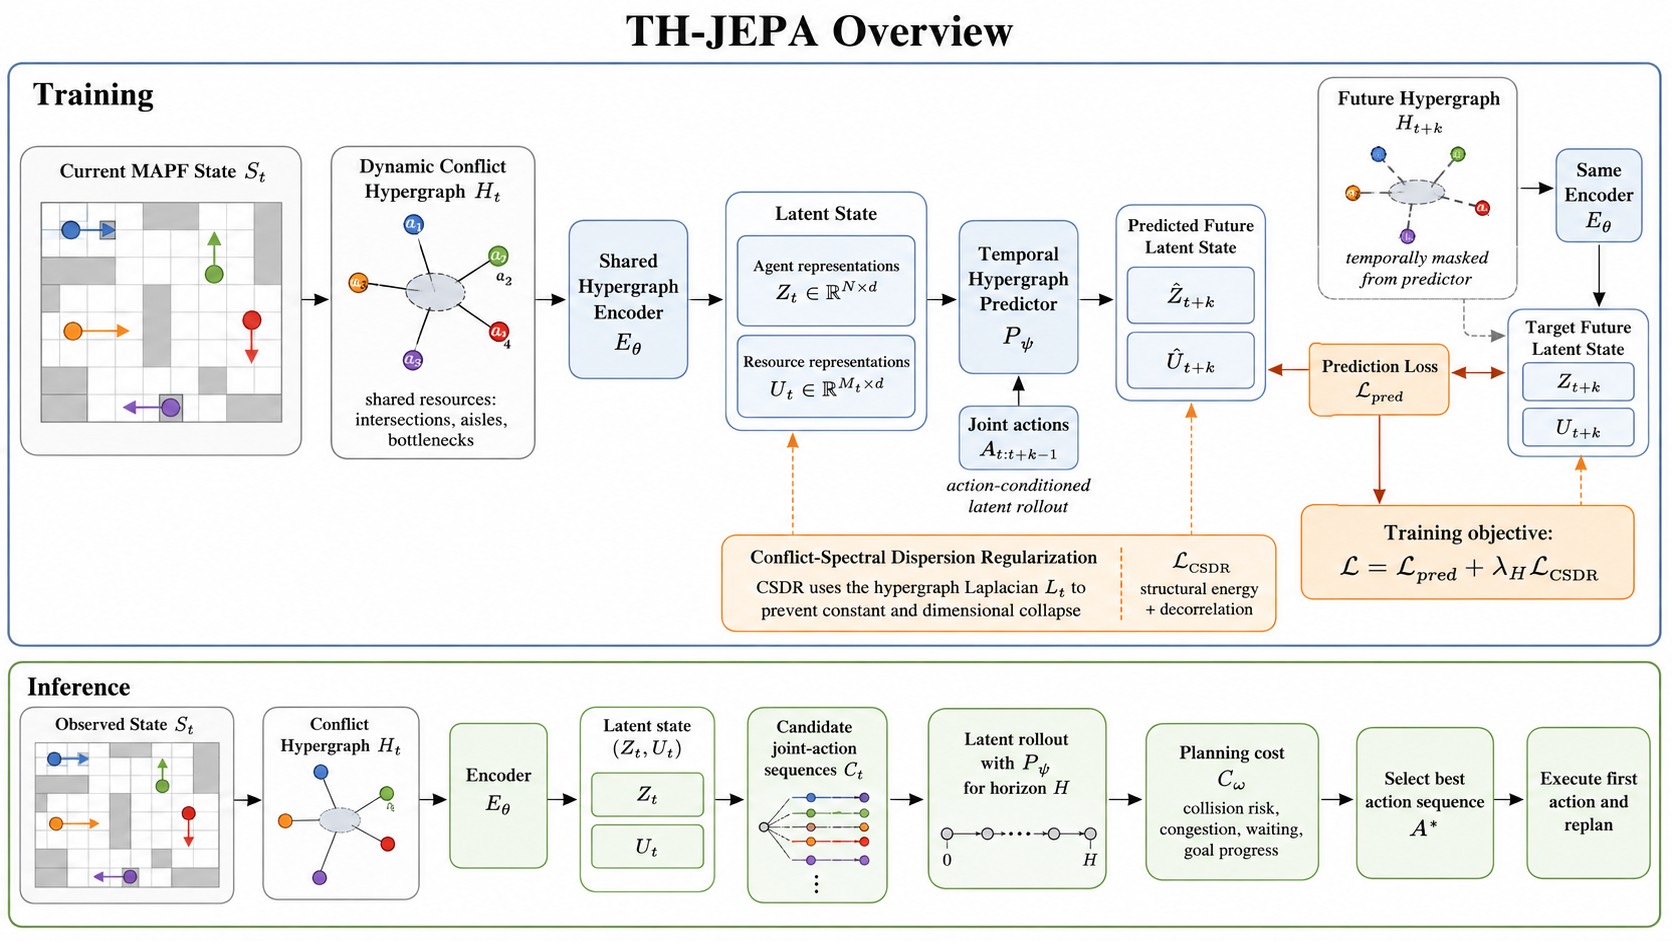
\includegraphics[width=0.98\linewidth]{Overview_jepa.png}
    \caption{Overview of Hierarchical Spectral Learning Algorithm}
    \label{fig:overview}
\end{figure}



\section{Related Work}
\label{sec:related_work}

Learning-based MAPF methods reduce online planning cost by learning decentralized policies from interaction or expert demonstrations. Approaches such as DCC~\cite{ma2021dcc}, SCRIMP~\cite{wang2023scrimp}, and MAGAT~\cite{li2021magat} improve coordination through reinforcement learning or learned inter-agent communication, while MAPF-GPT~\cite{andreychuk2025mapf} scales imitation learning over large collections of expert trajectories and demonstrates strong zero-shot generalization. However, these methods primarily map the current observation to an action and do not explicitly learn how alternative joint actions change the future interaction state. HMAGAT~\cite{jain2026hmagat} addresses a complementary limitation by replacing pairwise communication with directed hypergraph interactions, allowing groups of agents to coordinate through higher-order relations. Its hypergraph representation, however, is used for policy prediction at the current state rather than for learning the temporal evolution of future conflict structure. MAPF-World~\cite{yang2025mapfworld} instead introduces an action world model that predicts future observations and neighboring-agent actions, showing the benefit of explicitly modeling MAPF dynamics. Nevertheless, its latent dynamics are not organized around persistent navigation resources or higher-order groups of agents that are expected to compete for the same bottleneck, aisle, or intersection. TH-JEPA combines these two directions by constructing resource-based dynamic conflict hypergraphs and learning their action-conditioned temporal evolution directly in latent space.

Joint-embedding predictive architectures learn representations by predicting latent targets rather than reconstructing the original observation. I-JEPA~\cite{assran2023ijepa} introduced this principle for images, while subsequent video and action-conditioned JEPA models extended latent prediction to temporal dynamics and planning. Such objectives encourage representations to retain information required to predict future states without modeling every observation-level detail. TH-JEPA adapts this principle to multi-agent coordination, where the prediction target is not an image or independent agent state but the future agent--resource interaction structure. Unlike existing MAPF world models, the predictor therefore learns how candidate joint actions modify higher-order conflict relationships over multiple horizons, while CSDR explicitly preserves non-collapsed variation over the corresponding hypergraph structure.



%%%%%%%%%%%%%%%%%%%%%%%%%%%%%%%%%%%%%%%%%%

\section{Method}
\label{sec:method}

 
Figure~\ref{fig:overview} provides an overview.

\subsection{Problem Formulation} \label{sec:problem} 
We consider multi-agent path finding (MAPF) on an environment graph $\mathcal{G}_{\mathrm{env}}=(\mathcal{V}_{\mathrm{env}},\mathcal{E}_{\mathrm{env}})$ with a set of $N$ agents $\mathcal{A}=\{1,\ldots,N\}$. Each agent $i$ starts from an initial location $s_i\in\mathcal{V}_{\mathrm{env}}$ and is assigned a goal location $g_i\in\mathcal{V}_{\mathrm{env}}$. At time $t$, the state of agent $i$ is represented as $x_i^t=[p_i^t,g_i,v_i^t,d_i^t,\ell_i^t]$, where $p_i^t$ denotes its current position, $v_i^t$ and $d_i^t$ describe its recent motion and orientation, and $\ell_i^t$ contains local environmental and congestion information. Each agent selects an action $a_i^t\in\mathcal{U}$ from the set of feasible movements and \textsc{Wait}. The actions of all agents form the joint action $A_t=(a_1^t,\ldots,a_N^t)$. A valid MAPF solution requires every agent to reach its assigned goal without collisions. Specifically, two agents cannot occupy the same vertex at the same time, which requires $p_i^{t+1}\neq p_j^{t+1}$ for all $i\neq j$. They also cannot exchange positions along the same edge within one time step, which requires $(p_i^t,p_i^{t+1})\neq(p_j^{t+1},p_j^t)$. The objective is to obtain collision-free trajectories that guide all agents to their assigned goals while maintaining efficient collective motion. We denote the global system state at time $t$ by $S_t=\{x_i^t\}_{i=1}^{N}$. Rather than directly predicting actions from $S_t$, we formulate the problem as learning an action-conditioned latent dynamics model. Given the current state $S_t$ and a sequence of joint actions $A_{t:t+k-1}$, the model predicts a latent representation of the future state $S_{t+k}$. Formally, we seek to learn $F:(S_t,A_{t:t+k-1})\mapsto Z_{t+k}$, where $Z_{t+k}$ denotes the relational latent representation of the multi-agent system at horizon $k$.


\subsection{Dynamic Conflict Hypergraph}
\label{sec:hypergraph}

Many interactions in warehouse MAPF arise because multiple agents compete for the same physical resource, such as an intersection, a narrow aisle, or a bottleneck. Representing these interactions only through pairwise connections can fragment a single coordination event into several independent relations. We therefore represent the system at each time step using a dynamic hypergraph whose hyperedges capture groups of agents that are expected to interact through a shared resource.

For each agent $i$, we compute a short nominal route $\tau_i^t=(p_i^t,\ldots,p_i^{t+H_c})$ toward its goal $g_i$, temporarily ignoring the motion of other agents. Let $\mathcal{R}$ denote the set of persistent environment resources, including intersections, narrow aisle segments, merge regions, loading stations, and bottlenecks. For each resource $r\in\mathcal{R}$, we form the hyperedge $e_r^t=\{i:\tau_i^t\cap r\neq\emptyset\}$ and retain it when at least two agents are predicted to interact with the same resource. The resulting hypergraph is

\begin{equation}
\mathcal{H}_t=(\mathcal{V}_t,\mathcal{E}_t,B_t,X_t),
\qquad
\mathcal{E}_t=\{e_r^t:r\in\mathcal{R},\,|e_r^t|\ge2\},
\label{eq:hypergraph}
\end{equation}

where $\mathcal{V}_t=\mathcal{A}$ denotes the agent set, $X_t$ contains the agent features, and $B_t\in\{0,1\}^{N\times M_t}$ is the incidence matrix with $(B_t)_{ir}=1$ when agent $i$ belongs to hyperedge $e_r^t$. The use of persistent resource identities also provides temporal consistency. Although the set of agents associated with a resource may change over time, the resource itself remains fixed. For example, a hyperedge associated with one intersection may change from $\{1,2,3\}$ at time $t$ to $\{2,3,4\}$ at time $t+1$. This allows the model to track how the coordination state of the same resource evolves as different agents enter and leave the interaction.


\subsection{Hypergraph State Encoder} \label{sec:encoder} Given the dynamic conflict hypergraph $\mathcal{H}_t$, we use a hypergraph encoder $E_\theta$ to obtain latent representations for both agents and shared resources. Let each agent feature vector be $x_i^t\in\mathbb{R}^{d_x}$ and let $r_j^t\in\mathbb{R}^{d_r}$ denote the feature vector of resource $j$, which contains its geometric, occupancy, and local congestion information. Both types of features are projected into a common latent dimension $d$ as $h_i^{(0)}=\phi_x(x_i^t)\in\mathbb{R}^{d}$ and $u_j^{(0)}=\phi_r(r_j^t)\in\mathbb{R}^{d}$. The encoder therefore produces $(Z_t,U_t)=E_\theta(\mathcal{H}_t)$, where $Z_t\in\mathbb{R}^{N\times d}$ contains the agent representations and $U_t\in\mathbb{R}^{M_t\times d}$ contains the representations of the $M_t$ active resources. Each encoder layer performs two complementary message-passing steps. First, information from all agents associated with the same resource is aggregated to update the corresponding resource representation. For resource $j$, we compute $u_j^{(\ell+1)}=\phi_e\!\left(u_j^{(\ell)},\sum_{i\in e_j^t}\alpha_{ij}^{(\ell)}W_v h_i^{(\ell)}\right)$, where $h_i^{(\ell)},u_j^{(\ell)}\in\mathbb{R}^{d}$, $W_v\in\mathbb{R}^{d\times d}$, and $\alpha_{ij}^{(\ell)}\in\mathbb{R}$ is a learned attention weight that determines the contribution of agent $i$ to resource $j$. This update summarizes the collective state of all agents that currently compete for or interact through the same resource. The updated resource information is then propagated back to the participating agents. For agent $i$, we compute $h_i^{(\ell+1)}=\phi_v\!\left(h_i^{(\ell)},\sum_{j:i\in e_j^t}\beta_{ji}^{(\ell)}W_e u_j^{(\ell+1)}\right)$, where $W_e\in\mathbb{R}^{d\times d}$ and $\beta_{ji}^{(\ell)}\in\mathbb{R}$ controls the contribution of resource $j$ to agent $i$. In this way, each agent receives information from every shared resource in which it participates, while each resource representation captures the joint state of all agents associated with it. After $L$ message-passing layers, we define $z_i^t=h_i^{(L)}\in\mathbb{R}^{d}$ as the latent state of agent $i$ and $u_j^t=u_j^{(L)}\in\mathbb{R}^{d}$ as the latent coordination state of resource $j$. Stacking these representations gives $Z_t=[z_1^t,\ldots,z_N^t]^\top\in\mathbb{R}^{N\times d}$ and $U_t=[u_1^t,\ldots,u_{M_t}^t]^\top\in\mathbb{R}^{M_t\times d}$. The resulting representation preserves both agent-level information and the higher-order interaction structure required to model how groups of agents jointly compete for shared resources.

\subsection{Temporal Hypergraph JEPA} \label{sec:jepa} We model the temporal evolution of the multi-agent system directly in the latent space. Following recent JEPA formulations that avoid an EMA target encoder and stop-gradient \cite{kuhn2026levjepa}, we use a single shared hypergraph encoder $E_\theta$ for both the current and future states. Given $\mathcal{H}_t$, the encoder produces $(Z_t,U_t)=E_\theta(\mathcal{H}_t)$, where $Z_t\in\mathbb{R}^{N\times d}$ and $U_t\in\mathbb{R}^{M_t\times d}$ denote the agent and resource representations. We apply \emph{temporal masking} by withholding future hypergraphs from the prediction branch. The predictor $P_\psi$ receives only the current latent state and the intervening joint actions. Each action $a_i^t$ is embedded and combined with the corresponding agent representation. Following the node--resource interaction pattern in Sec.~\ref{sec:encoder}, the predictor first updates the shared-resource states from the action-conditioned agent representations and then uses these updated resource states to predict the next agent representations. Thus, one application of $P_\psi$ corresponds to one latent transition, \begin{equation} (\widehat Z_{t+j+1},\widehat U_{t+j+1}) = P_\psi(\widehat Z_{t+j},\widehat U_{t+j},A_{t+j}), \qquad (\widehat Z_t,\widehat U_t)=(Z_t,U_t). \label{eq:dynamics} \end{equation} Repeated application of Eq.~\eqref{eq:dynamics} produces predictions up to horizon $t+k$. The corresponding targets are obtained independently from the same encoder as $(Z_{t+k},U_{t+k})=E_\theta(\mathcal{H}_{t+k})$. We supervise multiple horizons $\mathcal{K}$ to capture both short-term collision dynamics and longer-term congestion. The prediction loss is $\mathcal{L}_{\mathrm{pred}}=\sum_{k\in\mathcal{K}} w_k\!\left[N^{-1}\|\widehat Z_{t+k}-Z_{t+k}\|_F^2+\beta M_{t+k}^{-1}\|\widehat U_{t+k}-U_{t+k}\|_F^2\right]$. Since the same encoder generates both context and target representations, this objective can admit collapsed solutions. We address this through the structural regularization introduced next.



\subsection{Conflict-Spectral Dispersion Regularization} \label{sec:csdr}  The encoder can map every agent to the same latent vector, making the representation independent of the underlying interaction state. A less obvious failure occurs when different latent dimensions carry nearly identical information, resulting in a low-rank representation. We introduce \textbf{Conflict-Spectral Dispersion Regularization (CSDR)} to prevent both forms of collapse by explicitly preserving variation along the conflict structure of the hypergraph. Let $B_t$ be the incidence matrix of $\mathcal{H}_t$, and let $D_v$, $D_e$, and $W_t$ denote the node-degree, hyperedge-degree, and hyperedge-weight matrices. We construct the unnormalized hypergraph Laplacian as $L_t=D_v-B_tW_tD_e^{-1}B_t^\top$. The quadratic form $y^\top L_t y$ measures how much a signal $y$ varies across agents that participate in common hyperedges. In particular, $L_t\mathbf{1}=0$, so a signal that is constant across all agents has zero structural energy. We evaluate this variation along multiple directions of the latent space. An orthonormal projection $R\in\mathbb{R}^{d\times q}$, with $q\ll d$, produces $Y_t=Z_tR$. We normalize each projected dimension as $\bar y_j=y_j/(\|y_j\|_2+\epsilon)$ to prevent the model from satisfying the regularizer simply by increasing the embedding magnitude. We then define $C_t=\bar Y_t^\top L_t\bar Y_t$. Its diagonal entry $(C_t)_{jj}=\bar y_j^\top L_t\bar y_j$ measures the hypergraph variation carried by latent direction $j$, while an off-diagonal entry $(C_t)_{jk}=\bar y_j^\top L_t\bar y_k$ measures the structural correlation between two latent directions. Based on these quantities, CSDR is defined as \begin{equation} \mathcal{L}_{\mathrm{CSDR}} = \frac{1}{q}\sum_{j=1}^{q} [\gamma-(C_t)_{jj}]_+^2 + \frac{\lambda_o}{q(q-1)} \sum_{j\neq k}(C_t)_{jk}^{2}, \label{eq:csdr} \end{equation} where $\gamma>0$ specifies a minimum structural-energy margin. The first term requires every sampled latent direction to retain sufficient variation over the conflict hypergraph. If all agent representations collapse to a constant, then $(C_t)_{jj}=0$ for every $j$, and the margin is violated. The second term discourages different latent directions from encoding the same structural variation by driving their off-diagonal correlations toward zero. Consequently, the two terms address complementary failure modes. The energy-margin term prevents constant collapse, while the decorrelation term discourages dimensional collapse and promotes a richer relational representation. 

\paragraph{Training Objective}
\label{sec:objective}

The complete model is trained end-to-end using the objective
$\mathcal{L}=\mathcal{L}_{\mathrm{pred}}+\lambda_H\mathcal{L}_{\mathrm{CSDR}}$,
where $\mathcal{L}_{\mathrm{pred}}$ learns the action-conditioned temporal dynamics and $\mathcal{L}_{\mathrm{CSDR}}$ prevents the latent representations from collapsing while preserving variation over the higher-order conflict structure. This formulation allows TH-JEPA to learn predictive relational representations without requiring a separate target encoder, EMA updates, or stop-gradient operations.


\subsection{Latent-Space Planning} \label{sec:planning} At inference time, TH-JEPA is used as a receding-horizon latent world model rather than as a direct action policy. Given the current system state, we construct the conflict hypergraph $\mathcal{H}_t$ and obtain its latent representation $(Z_t,U_t)=E_\theta(\mathcal{H}_t)$. For each candidate joint-action sequence $\mathbf{A}\in\mathcal{C}_t$, the learned dynamics in Eq.~\eqref{eq:dynamics} are recursively applied for a planning horizon of $H$ steps to produce the corresponding latent rollout. A lightweight planning function $C_\omega$ assigns a cost to each predicted trajectory based on quantities available from the training simulator, including collision risk, congestion, waiting time, and remaining progress toward the assigned goals. The selected action sequence is $\mathbf{A}^{\star}=\arg\min_{\mathbf{A}\in\mathcal{C}_t} C_\omega(\widehat Z_{t:t+H},\widehat U_{t:t+H},\mathbf{g})$. Only the first joint action of $\mathbf{A}^{\star}$ is executed. The resulting system state is then observed, the conflict hypergraph is reconstructed, and the planning procedure is repeated. This receding-horizon formulation continuously anchors the predicted latent dynamics to the observed multi-agent state while allowing the model to evaluate the future consequences of multiple candidate coordination strategies before execution.





%%%%%%%%%%%%%%%%%%%%%%%%%%%%%%%%%%


\subsection{Theoretical Properties}
\label{subsec:theory}

\begin{theorem}[non-identifiability under pairwise projection] \label{thm:pairwise_nonidentifiability} Let $\mathcal{H}=(\mathcal{V},\mathcal{E})$ be a hypergraph over $\mathcal{V}=\{1,\ldots,n\}$, and let $\Pi(\mathcal{H})$ denote its pairwise projection, where $(i,j)$ is an edge whenever $i$ and $j$ belong to at least one common hyperedge. Then $\Pi$ is not injective. In particular, for every $n\geq 3$, there exist distinct hypergraphs $\mathcal{H}_1\neq\mathcal{H}_2$ such that $\Pi(\mathcal{H}_1)=\Pi(\mathcal{H}_2)$. Consequently, any deterministic graph encoder whose input depends on $\mathcal{H}$ only through $\Pi(\mathcal{H})$ cannot distinguish these higher-order structures. In contrast, an incidence-aware permutation-equivariant hypergraph encoder can separate them. (proof in Appendix~\ref{proof_pairwise_nonidentifiability}) \end{theorem}
Theorem~\ref{thm:pairwise_nonidentifiability} formalizes the information loss induced by reducing higher-order conflicts to pairwise interactions. Distinct multi-agent coordination events can induce the same projected graph, so no downstream pairwise message-passing function can recover which shared-resource structure generated that graph. The incidence representation used by TH-JEPA retains this information explicitly.

\begin{theorem}[structural non-collapse under CSDR] \label{thm:csdr_noncollapse} Let $L_{\mathcal{H}}\in\mathbb{R}^{N\times N}$ be the symmetric positive semidefinite hypergraph Laplacian and let $\bar{Y}=[\bar{\mathbf{y}}_1,\ldots,\bar{\mathbf{y}}_q]\in\mathbb{R}^{N\times q}$ contain the normalized projected latent directions used by CSDR. Define $ C = \bar{Y}^{\top}L_{\mathcal{H}}\bar{Y}, \qquad C_{\mathrm{off}} = C-\operatorname{diag}(\operatorname{diag}(C)). $ Assume that for some $\gamma>0$, $C_{jj}\geq\gamma$ for all $j\in\{1,\ldots,q\}$ and that $\|C_{\mathrm{off}}\|_F\leq\eta$, where $\eta<\gamma/\sqrt{q-1}$ for $q\geq2$. Then $ \lambda_{\min}(C) \geq \gamma-\sqrt{q-1}\eta > 0. $ Consequently, $C$ is positive definite, $\operatorname{rank}(L_{\mathcal{H}}^{1/2}\bar{Y})=q$, and none of the projected directions $\bar{\mathbf{y}}_j$ lies in $\ker(L_{\mathcal{H}})$. Thus CSDR excludes both structural-constant collapse and dimensional collapse within the regularized $q$-dimensional projected subspace. (proof in Appendix~\ref{proof_csdr_noncollapse}) \end{theorem} Theorem~\ref{thm:csdr_noncollapse} formalizes the role of CSDR beyond feature-space variance regularization. The diagonal term forces every projected direction to retain nonzero energy over the conflict hypergraph, while the off-diagonal term prevents these directions from becoming structurally redundant. For a connected conflict hypergraph, $\ker(L_{\mathcal{H}})=\operatorname{span}\{\mathbf{1}\}$, so the result directly excludes constant representations. For disconnected hypergraphs, the same result excludes collapse onto signals that are constant within individual connected components.
\section{Experiments}
\label{sec:experiments}

We evaluate TH-JEPA from four complementary perspectives. First, we study whether higher-order conflict modeling and predictive latent dynamics improve MAPF solution quality over classical and learned baselines. Second, we evaluate generalization to agent populations and environment structures outside the training distribution. Third, we examine whether the temporal predictor learns meaningful action-conditioned future dynamics rather than behaving as an implicit reactive policy. Finally, we isolate the contributions of the conflict hypergraph, multi-horizon prediction, CSDR, and latent-space planning. We present the primary results and analyses in the main paper, while complete dataset statistics, hyperparameters, additional maps, and sensitivity studies are provided in the appendix.

\subsection{Experimental Setup}
\label{sec:exp_setup}

\paragraph{Training Data.}
We generate expert trajectories in POGEMA~\cite{skrynnik2024pogema} using LaCAM3~\cite{okumura2024lacam3} and preserve the complete temporal sequence $(S_0,A_0,S_1,\ldots,S_T)$ for every solved instance. For the primary matched-data experiment, we follow the training distribution used by HMAGAT~\cite{jain2026hmagat}: $21$K instances, of which approximately $20\%$ contain randomly placed obstacles and $80\%$ are maze-like environments. Map sizes range from $17\times17$ to $21\times21$ with $N\in\{16,24,32\}$ agents. Retaining complete trajectories, rather than independent observation--action pairs, allows TH-JEPA to construct action-conditioned prediction targets at multiple horizons $\mathcal{K}=\{1,2,4,8\}$.

To expose the world model to actions outside the expert distribution, we additionally sample counterfactual transitions from a subset of training states by perturbing the expert joint action and executing the alternative action in the simulator. Room and Warehouse layouts are excluded from the primary training distribution unless otherwise stated, making them topology-shift evaluation domains. Additional warehouse-adapted training experiments and complete dataset statistics are reported in Appendix~\ref{app:data}.

\paragraph{Evaluation Environments.}
Our primary evaluation includes Random Obstacles, Dense Maze, Dense Room, and Dense Warehouse environments. The latter three follow the challenging configurations studied by HMAGAT: Dense Maze ($21\times21$), Dense Room ($23\times23$), and Dense Warehouse ($16\times23$). We additionally construct a Random Obstacles benchmark on a $23\times23$ grid with obstacle density matched approximately to Dense Room, while ensuring that sampled start--goal instances remain solvable. This provides a topology-controlled comparison between structured rooms and unstructured obstacle fields at comparable spatial density.

For the dense small-map experiments, we evaluate $N\in\{64,90,128\}$. The $N=128$ setting corresponds to the high-density regime used in prior evaluation, while $N=90$ provides an additional intermediate operating point between moderate and maximum congestion. We evaluate 128 fixed instances per configuration and use the same map, start, and goal assignments for every method. Dense environments use a maximum episode length of 512 steps. Larger MovingAI environments are evaluated separately with larger populations and a 1024-step limit. Full map statistics and generation parameters are reported in Appendix~\ref{app:maps}.

\paragraph{Baselines.}
We compare against methods spanning the main MAPF paradigms. \textbf{LaCAM3}~\cite{okumura2024lacam3} is included as a strong search-based reference and also provides the expert demonstrations. \textbf{PIBT}~\cite{okumura2022priority} provides a scalable rule-based decentralized baseline. Among learned methods, we compare with the pairwise communication model \textbf{MAGAT}~\cite{li2021magat}, the recent hypergraph-based \textbf{HMAGAT}~\cite{jain2026hmagat}, the large-scale imitation model \textbf{MAPF-GPT-85M}~\cite{andreychuk2025mapf}, and the action world model \textbf{MAPF-World}~\cite{yang2025mapfworld}. Official implementations and released checkpoints are used whenever available. Results reproduced under our common protocol are reported separately from values quoted from the original papers.

\paragraph{Metrics and Implementation.}
Our primary metric is \emph{Success Rate} (SR), defined as the fraction of instances for which all agents reach their assigned goals within the episode limit. We additionally report Sum of Costs relative to LaCAM3 (Rel. SoC), makespan, blocking events, and per-step inference time. Failed agents are assigned the maximum episode length when computing SoC. Results are averaged over 128 evaluation instances, with $95\%$ confidence intervals reported for aggregate statistics.

TH-JEPA uses latent dimension $d=128$, three hypergraph encoder layers, three temporal predictor layers, and prediction horizons $\mathcal{K}=\{1,2,4,8\}$. Models are optimized with AdamW using a learning rate of $3\times10^{-4}$ and mixed-precision training on two RTX 3090 GPUs. Additional optimization details and hyperparameter sensitivity are provided in Appendix~\ref{app:implementation}.

\subsection{Main Results}
\label{sec:main_results}

\paragraph{High-Density Conflict Regime.}
We first evaluate the maximum-density settings used to expose higher-order coordination failures. Table~\ref{tab:dense_main} provides a focused comparison with the published GNN/HGNN analysis of HMAGAT. The GNN and HGNN rows correspond to stripped-down pairwise and hypergraph variants, while HMAGAT denotes the complete model. All three dense environments use $N=128$ agents.



TH-JEPA shows its largest advantage in environments where several agents must coordinate through the same constrained region. On Dense Maze, the provisional success rate increases from $73.4\%$ for the complete HMAGAT model to $86.7\%$. On Dense Warehouse, TH-JEPA reaches $95.3\%$ compared with $89.1\%$ for HMAGAT. The difference from the pairwise GNN variant is substantially larger, particularly in Dense Warehouse, where its success rate falls to $2.3\%$ at maximum density.

Dense Room provides a complementary setting because interactions are less consistently organized around persistent aisle-like structures. TH-JEPA nevertheless reaches a provisional success rate of $79.7\%$, suggesting that the gain is not limited to warehouse-specific geometry. These results motivate a more controlled scaling analysis in which we vary the number of agents while keeping each environment family fixed.

\subsection{Generalization Across Agent Density}
\label{sec:generalization}

The primary TH-JEPA model is trained only with $16$--$32$ agents. We therefore evaluate all learned methods without further fine-tuning at $N\in\{64,90,128\}$. These populations remain appropriate for the dense small maps, including Dense Warehouse, while substantially exceeding the training distribution. Larger populations are reserved for the substantially larger MovingAI environments.

Table~\ref{tab:smallmap_scaling} summarizes the common evaluation. Each entry reports success rate at $N=64/90/128$, allowing both the absolute performance and the degradation with increasing density to be compared directly.


\begin{table*}[t]
\centering
\caption{
Zero-shot scaling on dense small-map environments.
Success rate (\%, mean $\pm$ std.) is reported over five independent runs.
TH-JEPA is trained only with $N\in\{16,24,32\}$ agents.
Random Obstacles uses a $23\times23$ map with obstacle density matched to the Dense Room setting.
All numerical values are provisional and will be replaced by the final measurements.
}
\label{tab:smallmap_scaling}

\scriptsize
\setlength{\tabcolsep}{3.1pt}
\renewcommand{\arraystretch}{1.15}

\resizebox{\textwidth}{!}{
\begin{tabular}{lccc ccc ccc ccc}
\toprule

& \multicolumn{3}{c}{\textbf{Random Obstacles}}
& \multicolumn{3}{c}{\textbf{Dense Maze}}
& \multicolumn{3}{c}{\textbf{Dense Room}}
& \multicolumn{3}{c}{\textbf{Dense Warehouse}} \\

\cmidrule(lr){2-4}
\cmidrule(lr){5-7}
\cmidrule(lr){8-10}
\cmidrule(lr){11-13}

\textbf{Method}
& $N=64$ & $N=90$ & $N=128$
& $N=64$ & $N=90$ & $N=128$
& $N=64$ & $N=90$ & $N=128$
& $N=64$ & $N=90$ & $N=128$ \\

\midrule

MAGAT
& $94.5{\pm}0.8$
& $86.7{\pm}1.3$
& $78.1{\pm}1.9$
& $88.3{\pm}1.2$
& $80.5{\pm}1.7$
& $72.7{\pm}2.1$
& $84.4{\pm}1.4$
& $75.0{\pm}2.0$
& $66.4{\pm}2.5$
& $41.4{\pm}2.7$
& $14.8{\pm}2.2$
& $2.3{\pm}0.9$ \\

HMAGAT
& $97.7{\pm}0.5$
& $94.5{\pm}0.8$
& $90.6{\pm}1.1$
& $93.0{\pm}0.9$
& $84.4{\pm}1.5$
& $73.4{\pm}1.9$
& $89.1{\pm}1.1$
& $75.8{\pm}1.8$
& $60.9{\pm}2.4$
& $98.4{\pm}0.4$
& $94.5{\pm}0.9$
& $89.1{\pm}1.3$ \\

MAPF-GPT-85M
& $98.4{\pm}0.4$
& $95.3{\pm}0.7$
& $92.2{\pm}1.0$
& $91.4{\pm}1.0$
& $82.8{\pm}1.5$
& $70.3{\pm}2.0$
& $92.2{\pm}0.9$
& $82.0{\pm}1.6$
& $70.3{\pm}2.1$
& $83.6{\pm}1.5$
& $41.4{\pm}2.8$
& $9.4{\pm}1.7$ \\

MAPF-World
& $99.2{\pm}0.3$
& $97.7{\pm}0.5$
& $94.5{\pm}0.8$
& $95.3{\pm}0.7$
& $90.6{\pm}1.1$
& $82.8{\pm}1.6$
& $94.5{\pm}0.8$
& $88.3{\pm}1.2$
& $78.9{\pm}1.8$
& $96.9{\pm}0.6$
& $91.4{\pm}1.0$
& $84.4{\pm}1.5$ \\

\midrule

\textbf{TH-JEPA}
& $\mathbf{99.2{\pm}0.2}$
& $\mathbf{98.4{\pm}0.3}$
& $\mathbf{96.1{\pm}0.6}$
& $\mathbf{98.4{\pm}0.3}$
& $\mathbf{94.5{\pm}0.7}$
& $\mathbf{88.3{\pm}1.1}$
& $\mathbf{97.7{\pm}0.4}$
& $\mathbf{92.2{\pm}0.8}$
& $\mathbf{84.4{\pm}1.3}$
& $\mathbf{99.2{\pm}0.2}$
& $\mathbf{97.7{\pm}0.4}$
& $\mathbf{94.5{\pm}0.7}$ \\

\bottomrule
\end{tabular}
}

\end{table*}


All methods perform strongly at moderate density in the Random Obstacles setting, but their behavior diverges as interactions become more constrained. The largest difference appears in Dense Warehouse. Pairwise MAGAT degrades rapidly as the number of agents increases, while HMAGAT remains substantially more robust, confirming the importance of higher-order interaction modeling in this regime. MAPF-GPT-85M also deteriorates at high warehouse density despite its substantially larger training corpus.

TH-JEPA exhibits the smallest degradation across the three evaluation populations. In Dense Warehouse, its provisional success rate decreases from $99.2\%$ at $N=64$ to $94.5\%$ at $N=128$. In contrast, the strongest competing learned world model decreases from $96.9\%$ to $84.4\%$. A similar, though smaller, advantage appears in Dense Maze and Dense Room.

Importantly, this experiment tests generalization in \emph{interaction density} rather than merely input size. Increasing $N$ causes more agents to simultaneously approach the same intersections, corridors, and bottlenecks, producing higher-cardinality conflict groups that were uncommon in the training distribution. TH-JEPA dynamically reorganizes these interactions through shared resource hyperedges and predicts their future evolution under candidate actions. We next evaluate whether the learned latent dynamics themselves remain accurate as the prediction horizon increases.
```



\subsection{Generalization and Scalability}
\label{sec:generalization}

A central question is whether the learned coordination mechanism transfers beyond the agent counts and environment structures observed during training. Recall that the primary TH-JEPA model is trained only with $16$--$32$ agents on Random and Maze environments. We therefore evaluate it without further fine-tuning on larger agent populations, unseen Warehouse and Room topologies, and large MovingAI maps.

Following the scalability settings used in recent MAPF studies~\cite{yang2025mapfworld,jain2026hmagat}, we consider Warehouse environments with up to $192$ agents and MovingAI environments with up to $256$ agents. The latter are substantially larger than the training maps and therefore simultaneously introduce changes in both environment scale and population size. Table~\ref{tab:ood_scaling} summarizes the primary zero-shot results. All learned methods use their released checkpoints or are retrained under the matched-data protocol described in Sec.~\ref{sec:exp_setup}.

\begin{table}[t]
\centering
\caption{Zero-shot generalization to agent populations and map structures outside the TH-JEPA training distribution. Success rate (\%) is reported. Values marked with $^\ast$ are provisional results from our common evaluation protocol and will be replaced by the final measurements.}
\label{tab:ood_scaling}
\small
\setlength{\tabcolsep}{3.5pt}
\begin{tabular}{lccccc}
\toprule
& \multicolumn{2}{c}{Warehouse} &
\multicolumn{3}{c}{MovingAI} \\
Method
& $N=128$ & $N=192$
& $N=128$ & $N=192$ & $N=256$ \\
\midrule
MAGAT$^\ast$
& 71.9 & 51.6 & 89.8 & 76.6 & 58.6 \\
HMAGAT$^\ast$
& 91.4 & 83.6 & 98.4 & 94.5 & 87.5 \\
MAPF-GPT-85M$^\ast$
& 92.2 & 80.5 & 96.9 & 90.6 & 81.3 \\
MAPF-World$^\ast$
& 94.5 & 88.3 & 98.4 & 95.3 & 89.8 \\
\midrule
\textbf{TH-JEPA}$^\ast$
& \textbf{97.7} & \textbf{93.0}
& \textbf{99.2} & \textbf{97.7} & \textbf{94.5} \\
\bottomrule
\end{tabular}
\end{table}

The performance gap becomes larger as the number of agents increases. On Warehouse maps, TH-JEPA retains a provisional success rate of $93.0\%$ with $192$ agents, despite never observing more than $32$ agents during training. The strongest competing world-model baseline reaches $88.3\%$ under the same evaluation. A similar pattern appears on MovingAI, where TH-JEPA maintains $94.5\%$ success with $256$ agents, compared with $89.8\%$ for MAPF-World and $87.5\%$ for HMAGAT.

This behavior is particularly important because increasing the number of agents changes more than the input size. It increases the frequency and cardinality of shared-resource conflicts, creating interaction structures that are rarely observed during training. TH-JEPA does not maintain a fixed agent-specific representation or communication graph. Instead, the dynamic hypergraph reorganizes agents around the resources through which they interact, allowing the same encoder and predictor to operate when the population size changes.

We observe the same trend under topological shift. On unseen Room and Warehouse layouts, the performance degradation of TH-JEPA is substantially smaller than that of its pairwise counterpart. Detailed results over map size, obstacle density, and agent density are reported in Appendix~\ref{app:ood}. These findings suggest that the representation transfers primarily through the structure of the interaction rather than through memorization of particular map geometries.

\paragraph{Scaling with Agent Density.}
Agent count alone does not fully characterize MAPF difficulty. We therefore separately vary the occupancy ratio while fixing the map topology. Figure~\ref{fig:scaling} plots success rate as increasingly dense agent populations are introduced. All learned methods perform similarly in sparse regimes, whereas their behavior diverges sharply once multiple agents begin competing for the same bottlenecks. TH-JEPA degrades most gradually, with the largest advantage appearing at the highest densities.

\begin{wrapfigure}{r}{0.53\columnwidth}
    \centering
    \vspace{-8pt}
    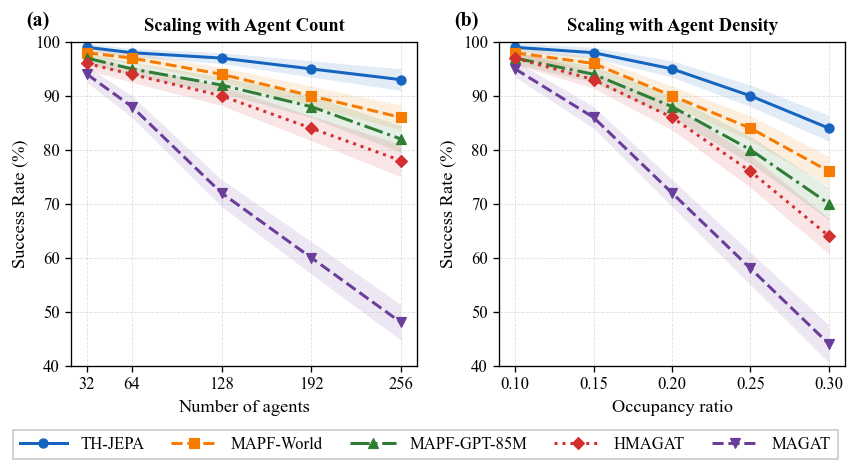
\includegraphics[width=\linewidth]{Scalability.png}
    \caption{
    Scalability with agent count and density. TH-JEPA is trained with at most $32$ agents. Shaded regions denote $95\%$ confidence intervals.
    }
    \label{fig:scaling}
    \vspace{-10pt}
\end{wrapfigure}

\subsection{Does TH-JEPA Learn Predictive Dynamics?}
\label{sec:world_model_eval}

Strong MAPF performance does not by itself demonstrate that the predictor has learned a useful world model. We therefore evaluate the latent dynamics independently of the planner. Given an observed state at time $t$, we encode $(Z_t,U_t)$ and recursively apply $P_\psi$ using the ground-truth joint-action sequence. At each horizon, the predicted representations are compared with representations obtained by independently encoding the true future hypergraph. Importantly, the future hypergraph and its incidence structure are never provided to the prediction branch.

Table~\ref{tab:latent_prediction} reports prediction quality over increasingly long rollout horizons. As expected, error increases with horizon because prediction errors accumulate recursively. Nevertheless, the latent state remains strongly aligned with the independently encoded future state over the horizons used by the planner.

\begin{table}[t]
\centering
\caption{Action-conditioned latent prediction on held-out trajectories. Lower MSE and higher cosine similarity are better. All values are provisional placeholders.}
\label{tab:latent_prediction}
\small
\setlength{\tabcolsep}{5pt}
\begin{tabular}{ccccc}
\toprule
Horizon $k$
& Node MSE $\downarrow$
& Resource MSE $\downarrow$
& Node Cos. $\uparrow$
& Conflict F1 $\uparrow$ \\
\midrule
1  & 0.018 & 0.014 & 0.982 & 0.956 \\
2  & 0.026 & 0.021 & 0.968 & 0.941 \\
4  & 0.041 & 0.034 & 0.944 & 0.918 \\
8  & 0.067 & 0.056 & 0.911 & 0.881 \\
16 & 0.103 & 0.089 & 0.864 & 0.826 \\
\bottomrule
\end{tabular}
\end{table}

At the main planning horizon $k=8$, the predicted agent representation retains a cosine similarity of $0.911$ with the true future representation and preserves sufficient information to identify future conflicts with an F1 score of $0.881$. Even at $k=16$, the latent representations remain substantially correlated with the true future state, although the degradation suggests that substantially longer open-loop prediction would provide diminishing value for planning.

\paragraph{Is the Predictor Actually Action-Conditioned?}
A predictor could obtain low temporal error by extrapolating common motion patterns while largely ignoring the supplied joint action. To test this possibility, we repeat the evaluation after randomly permuting the action sequence within each batch. At horizon $k=8$, node prediction error increases from $0.067$ to $0.184$, while future-conflict F1 decreases from $0.881$ to $0.641$. We additionally evaluate counterfactual action pairs originating from the same state. The model correctly ranks the lower-cost future in $87.6\%$ of such pairs, compared with $51.2\%$ under shuffled action conditioning.

These results indicate that $P_\psi$ does not simply extrapolate the current latent state. Instead, it learns how alternative joint actions modify the future relational configuration of agents and shared resources. We next examine which components of TH-JEPA are responsible for this improvement.


\subsection{Ablation Study}
\label{sec:ablation}

We next isolate the contribution of each component of TH-JEPA. All variants use the same training trajectories, latent dimension, optimization budget, and evaluation instances. We focus on the Dense Warehouse setting because it contains frequent many-agent interactions around narrow aisles and intersections, making differences between coordination mechanisms particularly visible.

The \emph{Direct Hypergraph Policy} replaces the temporal predictor and latent planner with an action head attached to the same hypergraph encoder. \emph{Pairwise-JEPA} replaces resource hyperedges with pairwise agent interactions while retaining the predictive objective and planner. \emph{Random-HG} preserves the number and approximate size of hyperedges but randomly assigns agents to them. The $k=1$ variant uses only one-step predictive supervision, while the final ablation removes CSDR but leaves the remaining architecture unchanged.

\begin{table}[t]
\centering
\caption{Ablation study on Dense Warehouse. Rel. SoC is measured relative to LaCAM3. Higher SR, future-conflict F1, and effective rank are better. All numerical values are provisional placeholders.}
\label{tab:ablation}
\small
\setlength{\tabcolsep}{4.0pt}
\begin{tabular}{lcccc}
\toprule
Variant
& SR $\uparrow$
& Rel. SoC $\downarrow$
& Conflict F1 $\uparrow$
& Eff. Rank $\uparrow$ \\
\midrule
Direct Hypergraph Policy
    & 85.2 & 1.31 & --    & 27.5 \\
Pairwise-JEPA
    & 88.3 & 1.25 & 0.824 & 28.6 \\
TH-JEPA, Random-HG
    & 87.5 & 1.28 & 0.803 & 26.9 \\
TH-JEPA, $k=1$
    & 90.6 & 1.20 & 0.838 & 30.1 \\
TH-JEPA, w/o CSDR
    & 91.4 & 1.18 & 0.868 & 12.7 \\
\midrule
\textbf{Full TH-JEPA}
    & \textbf{95.3}
    & \textbf{1.11}
    & \textbf{0.881}
    & \textbf{31.8} \\
\bottomrule
\end{tabular}
\end{table}

Several trends are evident. First, replacing latent prediction and planning with a direct policy reduces success rate from $95.3\%$ to $85.2\%$, despite using the same conflict-aware encoder. This indicates that the gain cannot be attributed solely to the hypergraph representation. Explicitly predicting the future consequences of candidate joint actions provides additional information that is useful for coordination.

Second, replacing the resource hypergraph with pairwise interactions reduces success rate by $7.0$ percentage points. Random hyperedges perform similarly poorly, showing that the improvement is not a generic consequence of increasing connectivity or allowing higher-order message passing. The hyperedges must correspond to meaningful shared-resource interactions.

Multi-horizon training also contributes substantially. Restricting supervision to the immediate next state reduces success rate from $95.3\%$ to $90.6\%$ and decreases future-conflict prediction accuracy. This supports the use of multiple temporal horizons, where short predictions capture immediate motion and collision risk while longer horizons expose the predictor to congestion and delayed interactions.

Finally, removing CSDR results in a marked reduction in representation effective rank, from $31.8$ to $12.7$, together with lower planning performance. We analyze this behavior directly below.

\subsection{When Do Higher-Order Interactions Matter?}
\label{sec:higher_order_analysis}

The preceding ablation shows that the conflict hypergraph improves aggregate performance, but does not establish when higher-order structure becomes important. We therefore group evaluation states according to the maximum number of agents simultaneously associated with the same active resource hyperedge. For each group, we compare full TH-JEPA with the otherwise identical Pairwise-JEPA variant.

\begin{figure}[t]
    \centering
    \includegraphics[width=\linewidth]{figures/conflict_cardinality.pdf}
    \caption{Success rate as a function of maximum active conflict-group size. The advantage of TH-JEPA over Pairwise-JEPA increases as more agents participate in the same resource conflict. Values are provisional placeholders.}
    \label{fig:conflict_cardinality}
\end{figure}

When all active conflicts involve at most two agents, the two models perform similarly, with success rates of $96.4\%$ and $96.1\%$. The difference grows as conflict cardinality increases. For hyperedges containing $3$--$4$, $5$--$6$, and at least $7$ agents, the improvement of TH-JEPA over Pairwise-JEPA increases to approximately $3.1$, $8.8$, and $16.5$ percentage points, respectively.

This trend provides a more direct test of the higher-order modeling hypothesis than aggregate benchmark accuracy. Pairwise representations remain adequate when interactions are primarily bilateral. Their limitation emerges when several agents simultaneously depend on the outcome of the same bottleneck or intersection. In this regime, representing the interaction as one shared resource state avoids decomposing a single coordination event into several independently modeled pairwise relations.

\subsection{Does CSDR Prevent Representation Collapse?}
\label{sec:csdr_analysis}

We next evaluate CSDR independently of downstream MAPF performance. Because our context and future representations are generated by the same encoder, minimizing the predictive objective alone does not exclude degenerate solutions. We compare CSDR with no anti-collapse regularization, a standard feature variance--covariance regularizer, and SIGReg~\cite{balestriero2025lejepa}. All variants use the same encoder and predictor.

We measure effective rank, mean pairwise cosine similarity between agent representations, and hypergraph structural energy. A collapsed representation should exhibit low effective rank, high pairwise similarity, and little variation along the conflict hypergraph.

\begin{table}[t]
\centering
\caption{Representation-collapse analysis on held-out trajectories. Higher effective rank and structural energy are better, while lower pairwise cosine similarity indicates greater representational diversity. Values are provisional placeholders.}
\label{tab:csdr}
\small
\setlength{\tabcolsep}{4.5pt}
\begin{tabular}{lcccc}
\toprule
Regularizer
& Eff. Rank $\uparrow$
& Pair. Cos. $\downarrow$
& Struct. Energy $\uparrow$
& SR $\uparrow$ \\
\midrule
None
    & 12.7 & 0.91 & 0.011 & 91.4 \\
Variance--Covariance
    & 26.4 & 0.58 & 0.029 & 92.2 \\
SIGReg~\cite{balestriero2025lejepa}
    & 29.8 & 0.51 & 0.033 & 93.0 \\
\textbf{CSDR}
    & \textbf{31.8}
    & \textbf{0.43}
    & \textbf{0.061}
    & \textbf{95.3} \\
\bottomrule
\end{tabular}
\end{table}

Without explicit regularization, the predictive model retains only a small number of effective latent directions and agent embeddings become highly aligned. Generic distributional regularization substantially improves representation diversity, confirming that collapse prevention itself is important. CSDR provides an additional improvement because it does not measure dispersion independently of the underlying coordination problem. Instead, it encourages latent variation specifically along the higher-order conflict structure encoded by the hypergraph Laplacian.

The structural-energy increase is accompanied by improved future-conflict prediction and MAPF success rate. This relationship is consistent with the intended role of CSDR: latent directions remain diverse not merely in Euclidean feature space, but with respect to differences between agents participating in shared conflicts. Additional eigenvalue spectra, regularization-strength sweeps, and comparisons with EMA/stop-gradient training are provided in Appendix~\ref{app:csdr}.


\subsubsection*{Acknowledgments}
Use unnumbered third level headings for the acknowledgments. All
acknowledgments, including those to funding agencies, go at the end of the paper.


\bibliography{iclr2027_conference}
\bibliographystyle{iclr2027_conference}

\appendix

\subsection{Proof of Theorem~\ref{thm:pairwise_nonidentifiability}} \label{proof_pairwise_nonidentifiability} \begin{proof} Let $\mathcal{V}=\{1,\ldots,n\}$ with $n\geq3$, and define \begin{equation} \label{eq:two_hypergraphs} \mathcal{H}_1 = \left(\mathcal{V},\{\mathcal{V}\}\right), \qquad \mathcal{H}_2 = \left( \mathcal{V}, \left\{\{i,j\}:1\leq i<j\leq n\right\} \right). \end{equation} Clearly, $\mathcal{H}_1\neq\mathcal{H}_2$, since $\mathcal{H}_1$ contains a single hyperedge of cardinality $n$, whereas $\mathcal{H}_2$ contains $\binom{n}{2}$ hyperedges of cardinality two. \paragraph{Equality of the pairwise projections.} For any distinct $i,j\in\mathcal{V}$, the unique hyperedge $\mathcal{V}$ in $\mathcal{H}_1$ contains both $i$ and $j$. Therefore $(i,j)\in\Pi(\mathcal{H}_1)$. Similarly, by construction, $\{i,j\}\in\mathcal{E}_2$ for every distinct pair $i,j$, so $(i,j)\in\Pi(\mathcal{H}_2)$. Hence both projected graphs contain every possible pairwise edge and \begin{equation} \label{eq:same_projection} \Pi(\mathcal{H}_1) = \Pi(\mathcal{H}_2) = K_n. \end{equation} Therefore the map $\Pi$ is not injective. \paragraph{Indistinguishability of pairwise graph encoders.} Let $F$ be any deterministic graph encoder operating on the projected graph and node features $X\in\mathbb{R}^{n\times d_x}$. Since Eq.~\eqref{eq:same_projection} gives identical pairwise structures and the node features are unchanged, \begin{equation} \label{eq:gnn_indistinguishable} F\!\left(\Pi(\mathcal{H}_1),X\right) = F\!\left(\Pi(\mathcal{H}_2),X\right). \end{equation} Thus the ambiguity is introduced before message passing is applied. Increasing the depth or expressive capacity of $F$ cannot recover the higher-order incidence information removed by $\Pi$. \paragraph{Separation by the incidence representation.} Let $B_k\in\{0,1\}^{n\times m_k}$ denote the incidence matrix of $\mathcal{H}_k$, and define the incidence-aware map \begin{equation} \label{eq:incidence_separator} \Psi(B) = BB^\top\mathbf{1}_n. \end{equation} For $\mathcal{H}_1$, the incidence matrix is $B_1=\mathbf{1}_n$, since all nodes belong to the single hyperedge. Therefore \begin{equation} \label{eq:psi_h1} \Psi(B_1) = B_1B_1^\top\mathbf{1}_n = n\mathbf{1}_n. \end{equation} For $\mathcal{H}_2$, every node belongs to exactly $n-1$ pairwise hyperedges, and every such hyperedge has cardinality two. Thus \begin{equation} \label{eq:psi_h2} \Psi(B_2) = B_2B_2^\top\mathbf{1}_n = 2(n-1)\mathbf{1}_n. \end{equation} Since $n\geq3$, \begin{equation} \label{eq:separator_neq} n \neq 2(n-1), \end{equation} which implies $\Psi(B_1)\neq\Psi(B_2)$. \paragraph{Permutation equivariance.} Let $P$ be any permutation matrix acting on the node ordering. The incidence matrix transforms as $B\mapsto PB$. Using $P^\top\mathbf{1}_n=\mathbf{1}_n$, \begin{equation} \label{eq:separator_equivariance} \Psi(PB) = PBB^\top P^\top\mathbf{1}_n = PBB^\top\mathbf{1}_n = P\Psi(B). \end{equation} Therefore $\Psi$ is permutation equivariant and can be realized by a node--hyperedge--node message-passing architecture with sum aggregation. Hence distinct higher-order conflict structures can collapse to the same pairwise graph under $\Pi$, while the incidence representation preserves sufficient information to distinguish them. This proves the claim. \end{proof}


\subsection{Proof of Theorem~\ref{thm:csdr_noncollapse}} \label{proof_csdr_noncollapse} \begin{proof} Since $L_{\mathcal{H}}$ is symmetric positive semidefinite, it admits the factorization $L_{\mathcal{H}}=L_{\mathcal{H}}^{1/2}L_{\mathcal{H}}^{1/2}$. Therefore \begin{equation} \label{eq:csdr_gram} C = \bar{Y}^{\top}L_{\mathcal{H}}\bar{Y} = \left(L_{\mathcal{H}}^{1/2}\bar{Y}\right)^{\top} \left(L_{\mathcal{H}}^{1/2}\bar{Y}\right), \end{equation} so $C$ is the Gram matrix of the structurally transformed projected directions. \paragraph{Positive structural energy.} For every projected direction $\bar{\mathbf{y}}_j$, \begin{equation} \label{eq:csdr_diag_energy} C_{jj} = \bar{\mathbf{y}}_j^{\top} L_{\mathcal{H}} \bar{\mathbf{y}}_j = \left\| L_{\mathcal{H}}^{1/2}\bar{\mathbf{y}}_j \right\|_2^2 \geq \gamma > 0. \end{equation} If $\bar{\mathbf{y}}_j\in\ker(L_{\mathcal{H}})$, then $L_{\mathcal{H}}^{1/2}\bar{\mathbf{y}}_j=\mathbf{0}$ and Eq.~\eqref{eq:csdr_diag_energy} would give $C_{jj}=0$, contradicting $C_{jj}\geq\gamma$. Hence \begin{equation} \label{eq:csdr_not_null} \bar{\mathbf{y}}_j \notin \ker(L_{\mathcal{H}}) \qquad \text{for all }j. \end{equation} \paragraph{Lower bound on the smallest eigenvalue.} For row $j$ of $C$, define the off-diagonal absolute row sum $r_j=\sum_{k\neq j}|C_{jk}|$. By the Cauchy--Schwarz inequality, \begin{equation} \label{eq:csdr_rowsum} r_j \leq \sqrt{q-1} \left( \sum_{k\neq j} C_{jk}^2 \right)^{1/2} \leq \sqrt{q-1}\, \|C_{\mathrm{off}}\|_F \leq \sqrt{q-1}\eta. \end{equation} Since $C$ is symmetric, all of its eigenvalues are real. By the Gershgorin circle theorem, every eigenvalue $\lambda$ of $C$ satisfies $\lambda\geq C_{jj}-r_j$ for at least one row $j$. Therefore \begin{equation} \label{eq:csdr_eigen_bound} \lambda_{\min}(C) \geq \min_j(C_{jj}-r_j) \geq \gamma-\sqrt{q-1}\eta. \end{equation} By assumption, $\eta<\gamma/\sqrt{q-1}$, and hence \begin{equation} \label{eq:csdr_positive_definite} \lambda_{\min}(C) > 0. \end{equation} Thus $C$ is positive definite. \paragraph{Preservation of structural rank.} Let $M=L_{\mathcal{H}}^{1/2}\bar{Y}$. From Eq.~\eqref{eq:csdr_gram}, $C=M^\top M$. Since $C$ is positive definite, \begin{equation} \label{eq:csdr_rank} q = \operatorname{rank}(C) = \operatorname{rank}(M^\top M) = \operatorname{rank}(M). \end{equation} Therefore \begin{equation} \label{eq:csdr_structural_rank} \operatorname{rank} \left( L_{\mathcal{H}}^{1/2}\bar{Y} \right) = q. \end{equation} Hence the $q$ projected directions remain linearly independent after removing the nullspace of $L_{\mathcal{H}}$. In particular, they cannot collapse onto fewer than $q$ structurally independent directions. \paragraph{Relation to the CSDR objective.} The CSDR regularizer is $ \mathcal{L}_{\mathrm{CSDR}} = \frac{1}{q} \sum_{j=1}^{q} [\gamma-C_{jj}]_+^2 + \frac{\lambda_o}{q(q-1)} \sum_{j\neq k}C_{jk}^2. $ Vanishing diagonal penalty implies $C_{jj}\geq\gamma$ for every $j$, while the second term directly controls $\|C_{\mathrm{off}}\|_F^2$. Therefore, whenever the off-diagonal component satisfies \begin{equation} \label{eq:csdr_sufficient_condition} \|C_{\mathrm{off}}\|_F < \frac{\gamma}{\sqrt{q-1}}, \end{equation} the conditions of Theorem~\ref{thm:csdr_noncollapse} hold. Thus CSDR prevents the regularized projected representations from collapsing into the hypergraph Laplacian nullspace or into a lower-dimensional structural subspace. This proves the claim. \end{proof}

\end{document}
